\documentclass[../main/thesis.tex]{subfiles}

\graphicspath{{/home/arefk/uio/MScThesis_AreKvanum2022_SeaIceML/thesis/datasets/figures/}}

\begin{document}
\section{Datasets}
[Training and validating a deep learning system requires data, which can be categorized in two distinct groups. The first group is the data known by the system, which is used during training to increase or validate model performance. Due to developing the model in such a way that it performs well against its validation data, external data is needed to validate the generalizability of the model. I.e., how well does the model perform with unknown data, which is assumed drawn from the same distribution as the data used during training. It is standard practice to arbitrarily split by a given fraction into the three datasets (training, validation, testing), as outlined above. However, due to the variable seasonal dependency of meteorological data, a naive split of the data could result in seasonally unbalanced datasets. As such, the datasets constructed for the purpose of this thesis are each covering at least a full year. Thus, no dataset is assumed to be skewed in the direction of any season.] \todo{Dette passer bedre inn i en train-test-split \textbf{model development}}

To facilitate the development and verification of a high resolution short-term deep learning sea ice forecasting system, several datasets covering observations and physical model forecasting systems have been chosen. When selecting appropriate datasets, their spatial resolution as well as release frequency has been considered. Even though several observational sea ice concentration products exists which cover the region of interest (see Figure \ref{fig:studyarea}), a lot of the satellite products based on passive microwave retrievals are of a too coarse resolution (e.g. \citet{Lavergne2019} or \citet{Kern2019}) to be able to aid in short term decision making \citep{Wagner2020}. On the other hand synthetic aperture radar (SAR) observations such as Sentinel 1A Interferometric Wide swath ($5\text{m} \times 20\text{m})$ or Extra-Wide swath ($20\text{m} \times 40\text{m}$) are on a structure resolving spatial resolution. However the daily SAR coverage is sparse in the Arctic (See Supporting Figure \ref{fig:S-sar}) and there are currently no maps made from automatic sea ice concentration retrieval algorithm from SAR observations which are known to the author.

Moreover, forecasts provide the deep learning system with information regarding how the domain will evolve in the period after the forecast has been initialized. Thus allowing the deep learning system to also rely on the forecasted development of the system when making decisions. Hence, atmospheric variables from a regional numerical weather prediction system will be included as input to the model, which encodes information about the future sea ice state through the variables correlation to the sea ice concentration.

Finally, the highest resolution product with an appropriate temporal frequency available are the sea ice charts produced by the NIS \citep{Dinessen2020}. Moreover, the sea ice charts represents an interpretation of different sea ice observations delivered as product directed towards operational users. Thus, the sea ice charts will serve as the ground truth for the model. Furthermore, as a deep learning system can increase its skill by combining correlated variables as input, this thesis will explore the impact caused by including several datasets covering both current observations, past trends as well as forecasted variables on different spatial resolutions as input predictors.

The following section will describe the domain covered for this thesis, followed by a rundown of the satellite products as well as physical models used. Table \ref{tab:data_overview} presents the different products used for this thesis, and whether the product is used to train or verify the model.

\begin{table}[]
    \caption{\label{tab:data_overview}Rundown of the products used and their applications. The dashed line separates observational products (above) from forecast products (below)}
    \centering
    \setlength{\arrayrulewidth}{0.5mm}
    \renewcommand{\arraystretch}{1.3}
    \begin{tabular}{llll}
    \hline
    Product             & Variables           & Training & Verification \\
    \hline
    Ice charts          & SIC                 & Yes      & Yes          \\
    OSI-SAF SSMIS       & SIC trend           & Yes      & Yes          \\
    OSI-SAF CDR         & Ice edge length     & No       & Yes          \\
    AMSR2               & SIC                 & No       & Yes          \\
    \hdashline
    AROME-Arctic        & T2M, X-wind, Y-wind & Yes      & No           \\
    NeXtSIM             & SIC                 & No       & Yes          \\
    Barents-2.5         & SIC                 & No       & Yes          \\
    \hline         
    \end{tabular}
\end{table}


\subsection{Region}
The domain covered by the deep learning system, covers part of the European Arctic. The region is an intersection between the domain covered by the Ice Charts \citep{Dinessen2020} and AROME Arctic \citep{Mueller2017} as shown in Figure (\ref{fig:studyarea}). The domain has a 1km spatial resolution, and contains $1972 \times 1972$ equidistant grid points. Compared to the AROME Arctic grid, the model domain has a reduced southern and eastern extent, which is manually subsectioned to conform to the square grid imposed by the deep learning architecture \citep{Ronneberger2015}. Another reason for the reduced domain extent was to limit the amount of memory needed when loading data during training. Both reasons will be thoroughly discussed in later sections. Moreover, the choice of limiting the southern and eastern extent of the domain was deliberate to reduce the amount of likely sea ice concentration containing grid cells lost in the process.

\begin{figure}
    \centering
    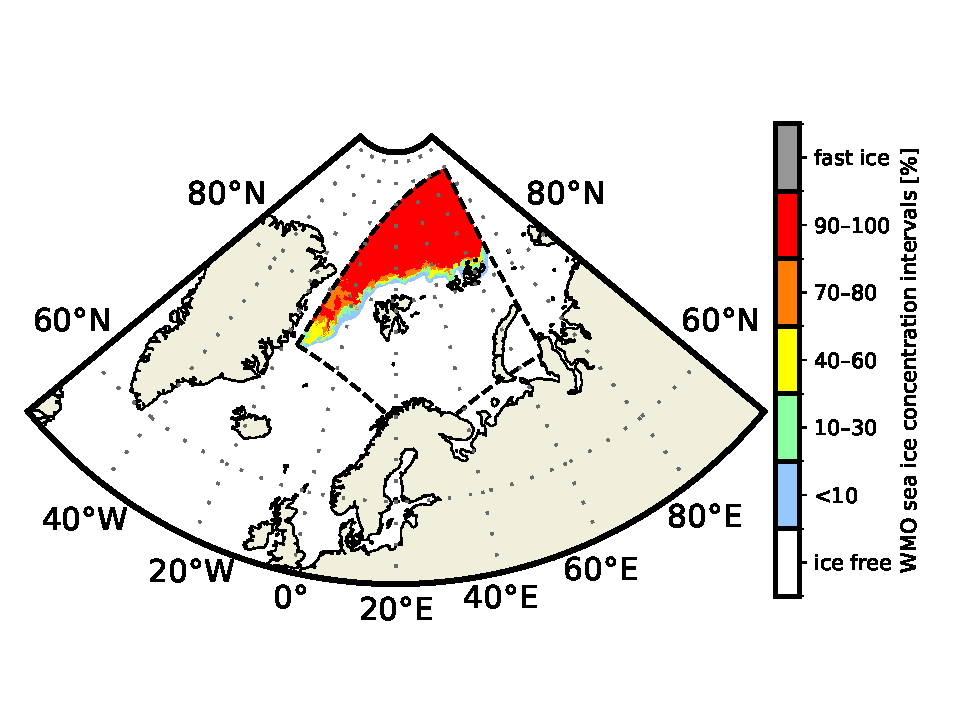
\includegraphics[width = 0.7\textwidth]{study_area}
    \caption{\label{fig:studyarea}The model domain is shown by sea ice concentration contours retrieved from a sea ice chart (15 Sep 2022). No colorbar is shown, light blue is free open water and yellow is fast ice. Land is displayed atop the domain for visualization purposes only.}
\end{figure}

\subsection{Observations}
Observations are used to convey the current state of sea ice concentration. There is a lack of consistent in situ observations of sea ice concentration, due to the remoteness of the region. Thus, most independent observations are ship-based concentration estimates \citep{Kern2019} or optical remote sensing, the latter is only available during summer. As a result, sea ice concentration is mainly observed automatically through passive microwave retrievals utilizing different sea ice retrieval algorithms \citep{Lavergne2019a, Comiso1997,Spreen2008}. Another source of sea ice observations are sea ice charts (\url{https://usicecenter.gov/}, Last Accessed 25 Jan 2023) \citep{Dinessen2020}, which are manually drawn interpretations combining available sea ice concentration observations such as SAR, passive microwave and optical imagery. 

\subsubsection{Sea Ice Charts}
The sea ice charts utilized for this thesis are provided by the Norwegian Meteorological Institute through the National Ice Service. The product is manually drawn by a sea ice specialist, and is distributed every workday at 15:00 UTC. The Sea Ice specialist assesses available SAR data from Sentinel 1 and Radarsat 2. However, due to the spatial variability in daily SAR coverage (See Supporting Figure (\ref{fig:S-sar})), visual, infrared and low resolution passive microwave observations are supplied to achieve a consistent spatial coverage \citep{Dinessen2020}. The sea ice charts are not drawn onto any resolution. Hence, a gridded representation of the ice charts is only a representation of the mean value of the polygons contained inside each grid cell. The sea ice charts accessed in this work has been interpolated onto the same projection as AROME Arctic \citep{Mueller2017}, and is presented on a 1km spatial grid.

With regards to consistency, it is noted that the current sea ice chart product used have no easily identifiable way of noting which observations were used by the sea ice analyst to draw each segment of the chart. As the different satellite products used pose different spatial scales, from meters to kilometers \citep{Dinessen2020}, the underlying uncertainty and ability to resolve structures varies both spatially and temporally. The published sea ice charts as seen in Figure (\ref{fig:icechart}) visualize the available SAR coverage, which is the preferred data source of the ice analysts \citep{Dinessen2020}. 

\begin{figure}
    \centering
    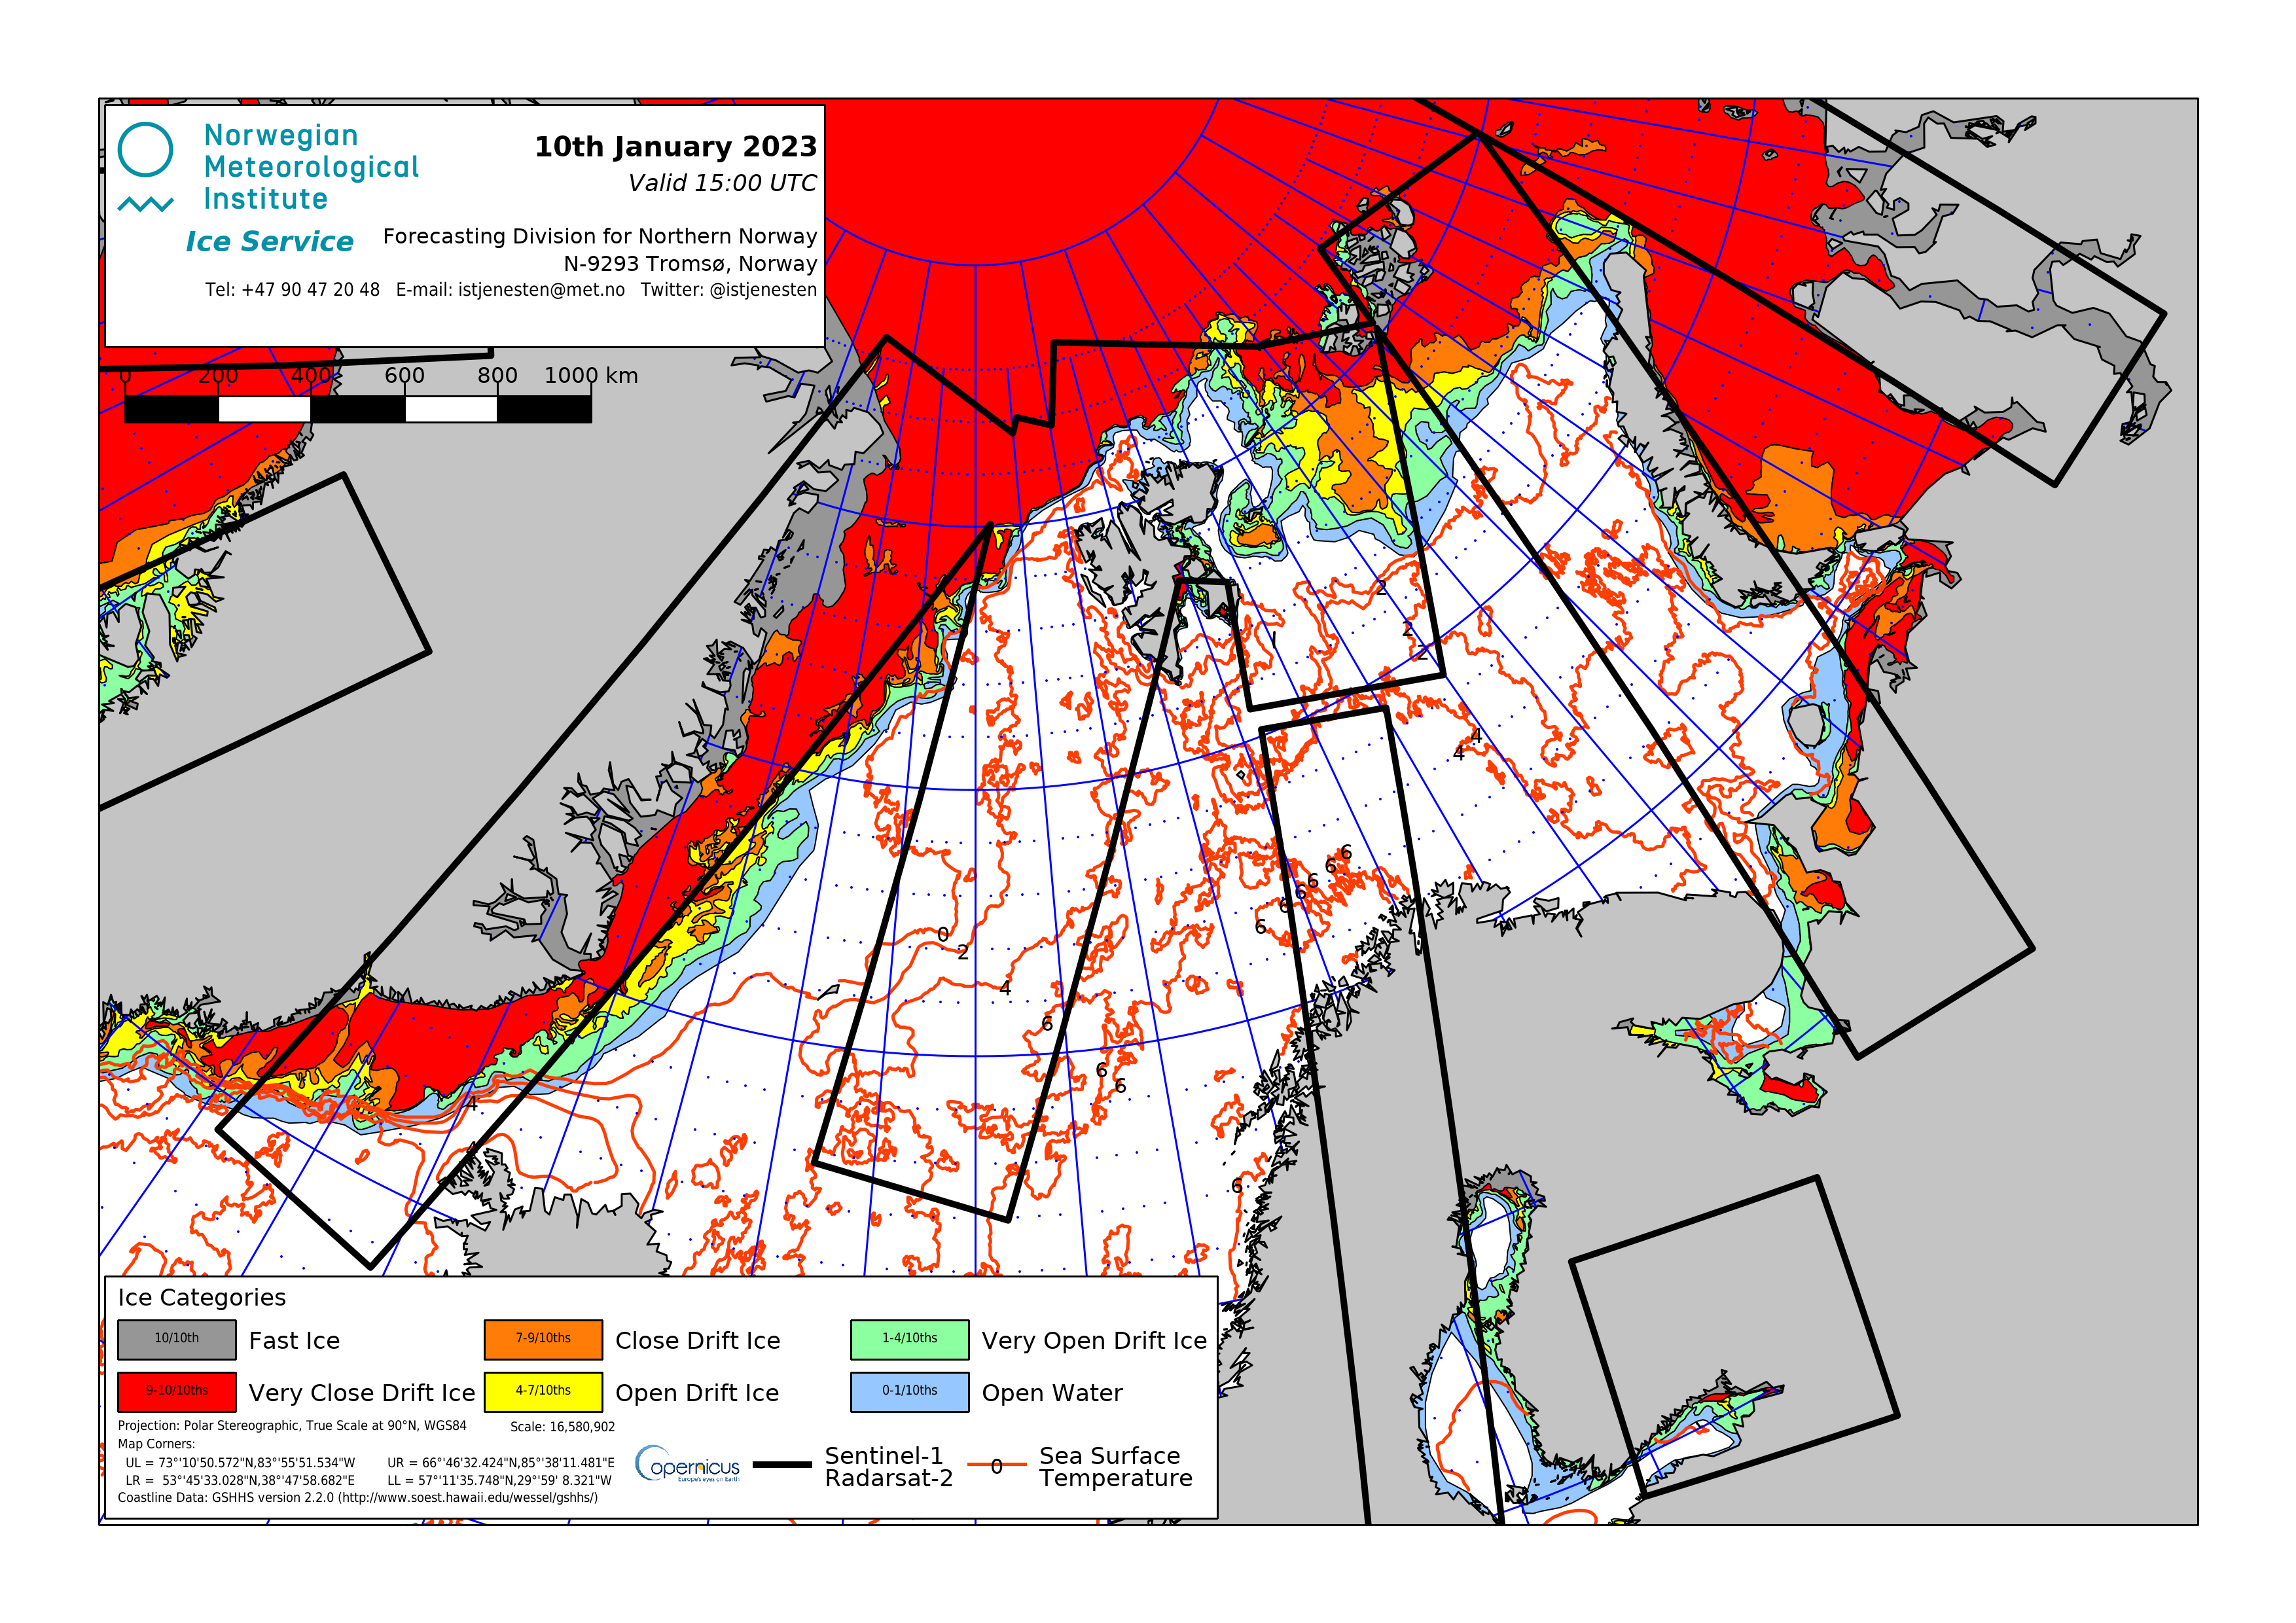
\includegraphics[width=0.9\textwidth]{general_latest}
    \caption{\label{fig:icechart}Sea Ice chart produced by the NIS covering 10 Jan 2023 at 15:00 UTC. Sea ice concentration categories are drawn as filled contours. The black lines indicate the available SAR data used to draw the sea ice chart.}
\end{figure}

\begin{figure}
    \centering
    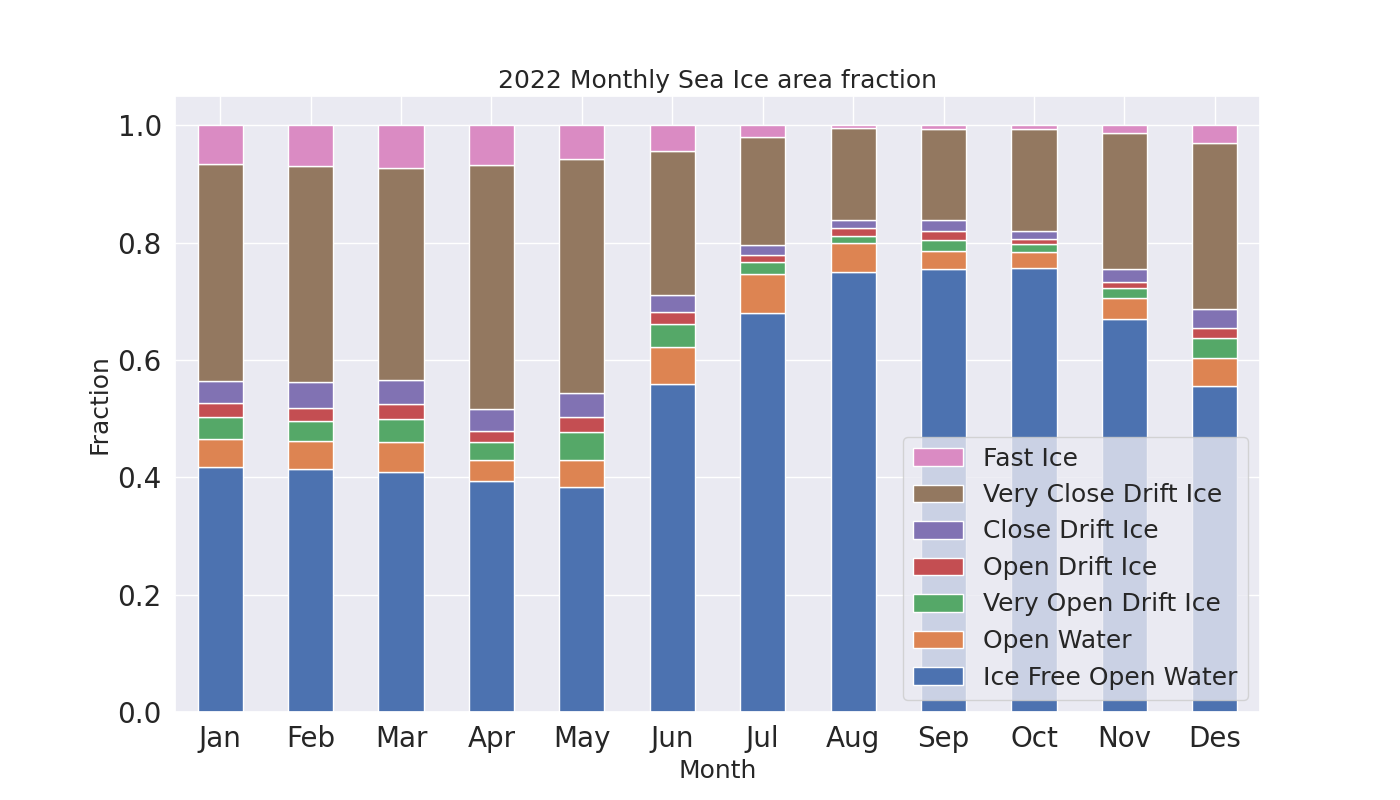
\includegraphics[width=0.8\textwidth]{2022-sic-distribution}
    \caption{\label{fig:2022-areadist-sic}Monthly distribution of each concentration class as respective fraction of the total mean sea ice concentration for the sea ice charts covering 2022. \textbf{[Could extend to cover larger time period (e.g. from 2011), give a more climate perspective of the sea ice evolution], Add concentration ranges for each class}}
\end{figure}

Figure (\ref{fig:2022-areadist-sic}) shows the monthly distribution of sea ice concentration contours from the sea ice charts during the period of 2022. As can be seen from the figure, almost half of the region consists of ice free open water, with the other majority of an ice chart consisting of very close drift ice. Moreover, the figure shows the seasonal variability of the sea ice extent, with the ice free open water constituting $\sim60$\% of the entire domain. The ice charts also resolve the intermediate sea ice concentration classes, which for the current region is mostly related to the marginal ice zone and the ice edge.

\begin{figure}
    \centering
    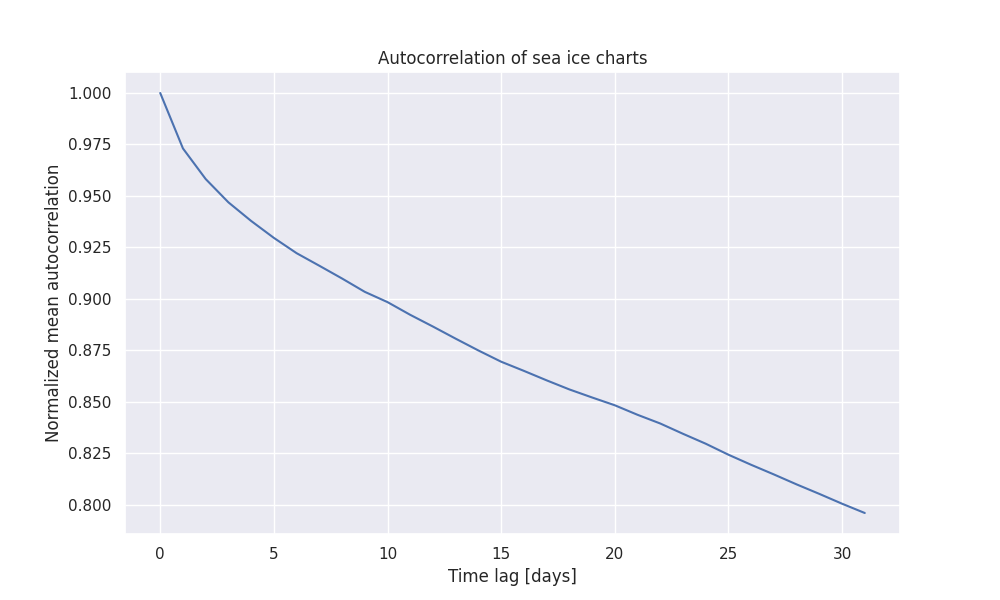
\includegraphics[width = 0.8\textwidth]{autocorr_icechart}
    \caption{\label{fig:autocorr}Autocorrelation of the sea ice charts from 2022. The x-axis is the time lag between to entries 2022 sea ice chart timeseries. The y-axis is the normalized autocorrelation, i.e. autocorrelation at a certain time lag divided by the autocorrelation at time lag 0. The autocorrelation is computed for a period covering 31 days.}
\end{figure}

By inspecting Figure (\ref{fig:autocorr}), it can be seen that the autocorrelation between two ice charts close in time is high. However, it can also be seen to steadily decline as the time lag increases. From the strong autocorrelation seen in Figure (\ref{fig:autocorr}), it can be assumed that persistence forecasting for short lead times (days) aptly describe the sea ice concentration development. Furthermore, the autocorrelation also renders previous sea ice concentration at short timescales as skillful at describing the current growth of the sea ice. The latter will be used as motivation to compute a sea ice concentration trend in a coming subsection.

The Sea Ice charts is an operational product aimed at marine end users. This influences the decision-making when creating the final operational product. Furthermore, though a single ice chart is assumed to be drawn by the same person, there are several sea ice specialists at the NIS whom draw ice charts. Hence, it can be assumed that there is an unknown degree of personal bias to data. On the other hand, the human involvement may also introduce a degree of quality control not seen in automatic sea ice concentration retrieval algorithms. Thus, the ice charts are assumed to have a low uncertainty, though there are no uncertainty estimates included \citep{Dinessen2020}.

In spite of the uncertainties outlined above, the sea ice charts are assumed to be the most accurate sea ice concentration product available for the purpose of high resolution data tailored towards operational end users. Through utilizing the sea ice charts as the ground truth data when training the deep learning system, the developed model will fit towards the high resolution operational use case proposed.

\subsubsection{Osi-Saf}
Two different Sea Ice Concentration products are used from OSI-SAF. OSI-SAF SSMIS is an operational product delivering daily sea ice concentration on the northern (and southern) hemisphere. OSI-SAF Climate Data Record (CDR) \citep{Soerensen2021} deliver sea ice climatology beginning in 1979 \citep{Lavergne2019} The operational product will be used as a predictor for the model and for validation, whereas the climatology will be used only for validation purposes only. 

\textbf{OSI SAF SSMIS}

OSI-SAF SSMIS is a passive microwave product derived from the Special Sensor Microwave Imager and Sounder (SSMIS). To convert brightness temperature to estimated sea ice concentration, a hybrid approach combining the Bootstrap algorithm \citep{Comiso1997} and the Bristol algorithm \citep{Smith1996} where the prior is used over open water and the latter used for ice concentrations above 40\% \citep{Tonboe2017}. The algorithm uses data from the 19GHz frequency channel (Vertically polarized) and 37GHz channel (Vertically and Horizontally polarized), which are the two lowest sprectral resolution channels for the SSMIS \cite{Tonboe2017}. The end product is on a 10km polar stereographic grid.

With regards to uncertainty, OSI SAF SSMIS is validated against pan-arctic sea ice charts from the U.S. National Ice Center as well as regional sea ice charts covering the Svalbard region from the NIS. Moreover, the operational product is required to have a bias and standard deviation less then 10\% ice concentration on an annual basis, when compared to the mentioned targets (\url{https://osisaf-hl.met.no/sea-ice-conc-edge-validation}, Last Accessed 24 Jan 2023). This strengthens the previously made statement that sea ice charts are low-uncertainty products.

The operational OSI-SAF SSMIS data is used to compute a coarse resolution (with respect to the ice charts) linear sea ice trend in each grid cell, with a length of 3 to 7 days. The idea behind the computed trend is to encode multiple time-steps of sea ice concentration fields into a single 2d-array, in line with the lack of temporal awareness of the deep learning architecture as well as the limiting the amount memory needed as information from multiple large arrays are contained in a single field. Furthermore, the ice concentration trend is computed from a separate sea ice product than the ice chart, with the intent to supply the model with correlated but not overlapping information, as the current day ice chart is already used as a predictor. However, it should also be noted that the lack of sea ice charts during the weekends \citep{Dinessen2020} is also a contributing factor, since the daily frequency results in a complete dataset and allows for trends consisting of $>5$ days to be computed. The coarser resolution also contribute to the OSI-SAF trend serving as complementary information to the ice charts, as the coarse resolution make the trend less resolvent of the local variability which is seen in the ice charts. As such, the trend serves as a indicator of where the sea ice growth is occurring.

The temporal length used when deriving trend will have an impact as to how accurate the computed trend reflects the current growth and retreat zones, especially with regards to the volatile position of the ice edge on a daily timescale but also due to the seasonal variability of the ice area \citep{Holland2016}. Hence, a too large lookbehind would cause a decorrelation between the current sea ice concentration and computed trend. On the other hand, Figure (\ref{fig:autocorr}) shows that there exist a significant autocorrelation for sea ice concentration on a short time-range, as described previously.

\textbf{OSI SAF Climate Data Record}

As briefly mentioned in Section (\ref{sec:introduction}), OSI-SAF Climate Data record combines observations from different sensors (SMMR, SSM/I, SSMIS) as well as numerical weather prediction fields from the ERA Interim reanalysis \citep{Dee2011}. The latter are utilized to correct for the atmospheric conditions. Two versions of the dataset has been used, version 2 (OSI-450) which covers (2011 - 2015), and the interim version (OSI-430-b) which cover (2016 - 2020) (\url{https://osisaf-hl.met.no/osi-450-430-b-desc})(Last Accessed 18 Jan 2023). Both products are processed using the same algorithms, ensuring consistency \citep{Lavergne2019a}. The Interim version is serving as an extension of the original scope of OSI-450 (1979 - 2015), with a difference being its use of ECMWF weather forecasts data compared to the reanalysis and different SSMIS input data (\url{https://osisaf-hl.met.no/osi-450-430-b-desc}, Last Accessed 24 Jan 2023). Regardless, both products will hereby be referred to in tandem as OSI SAF CDR

The OSI SAF retrieval algorithm has been shown to have strong correlation against ship based measurements \citep{Kern2019} as well as optical satellite observations during the summer \citep{Kern2020}. Hence, OSI SAF CDR is expected to serve as a correct representation of the Arctic sea ice concentration, however it is noted that no retrieval algorithm is able to match the true state of the sea ice concentration.

OSI SAF CDR is provided with a 25km spatial resolution on a Lambert Azimuthal Grid projection \citep{Soerensen2021}. The sea ice concentration data retrieved has been used to compute a climatological ice edge length for each day of the year, applying a daily mean across the time period (2011 - 2020). The ice edge length has been computed according to \citep{Melsom2019}, which will be derived in Section (not yet labelled). Note that though OSI SAF CDR provide a pan-arctic distribution of sea ice concentration, the data has been regridded onto the study region domain with the  AROME Arctic projection and a 25km grid spacing before computing the ice edge length.

\begin{figure}
    \centering
    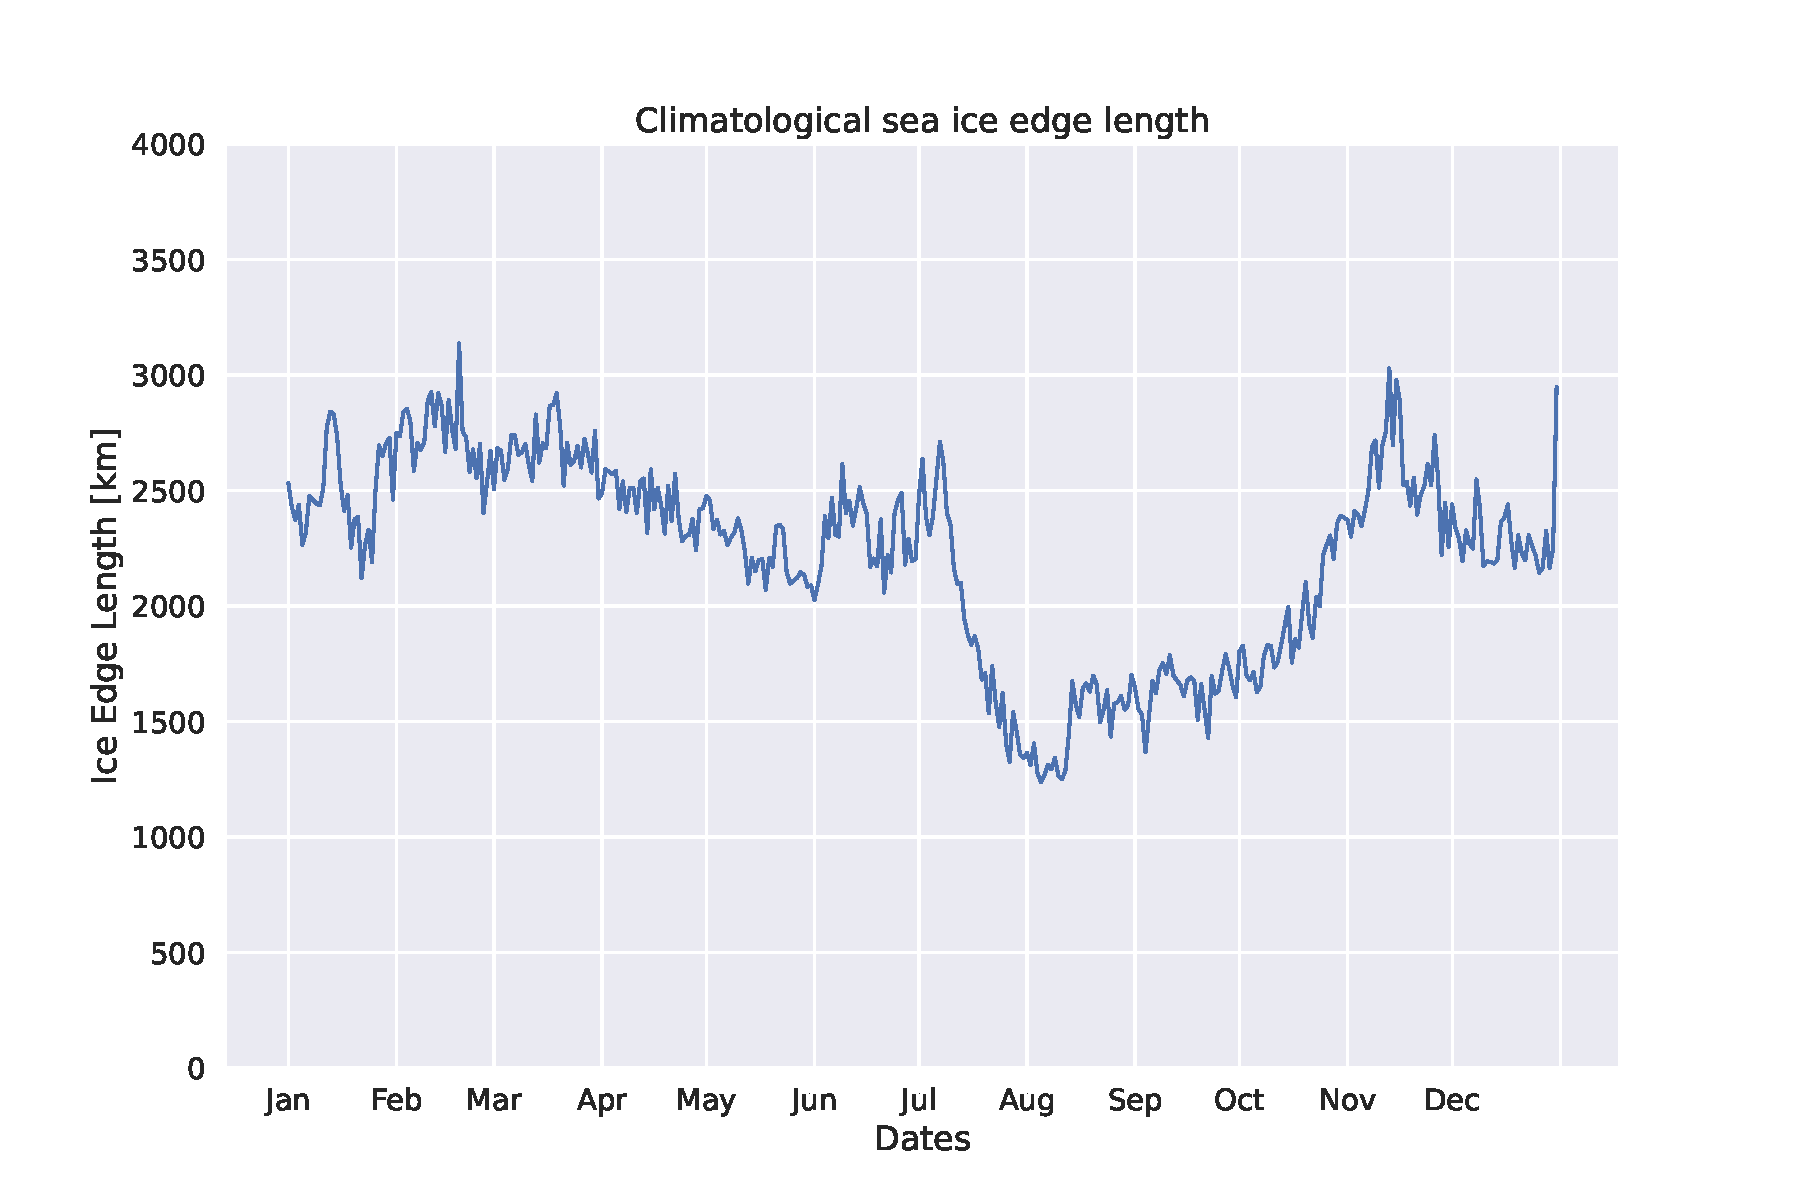
\includegraphics[width = 0.7\textwidth]{clim_iceedge}
    \caption{\label{fig:clim_iceedge} \textbf{FIX NONSENSICAL XTICKLABELS} Seasonal variability of the Arctic climatological ice edge length computed from satellite observations during the period 2011 - 2020}
\end{figure}

As can be seen in Figure (\ref{fig:clim_iceedge}), the Arctic sea ice edge experiences a strong seasonal variability. The computed climatological ice edge will be used as a normalization factor to ensure that the seasonal influence on ice edge length dependant verification scores is mitigated \citep{Goessling2016, Zampieri2019, Palerme2019}. Another benefit from utilizing a single ice edge length is to ensure that different sea ice products are normalized according to a common and independent sea ice length. Furthermore, it will be shown in a later section that the Integrated Ice Edge Error \citep{Goessling2016} (Not yet derived) normalized by the ice edge length is correlated with the resolution of the ice edge length, proving the validity of normalizing using a common, coarse resolution ice edge length.

\subsubsection{AMSR2}
The Advanced Microwave Scanning Radiometer 2 (AMSR2) data utilized for this thesis is the sea ice concentration product from the University of Bremen (\url{https://seaice.uni-bremen.de/sea-ice-concentration/amsre-amsr2/})(Last Accessed 18 Jan 2023). AMSR2 is a passive microwave sensor observing the microwaves emitted by the Earth, similar to \textbf{OSI SAF SSMIS}. AMSR2 is located on the JAXA GCOM-W1 satellite \cite{Melsheimer2019}, and is retrieved using the ASI algorithm \cite{Spreen2008}. The algorithm uses data from the 89GHz channel, which is the band posing the highest spectral resolution, in both polarizations to determine the sea ice concentration. Bands at lower spectral resolutions are only used as weather filters, which can mask out false sea ice detected in the open ocean \cite{Spreen2008}. The resulting data is a pan-arctic sea ice coverage with a spatial resolution of 6.25km.

The current AMSR2 product was chosen as the ASI retrieval algorithm \citep{Spreen2008} results in a higher spatial resolution product compared to similar AMSR2 products such as the AMSR2 product from OSI SAF \citep{Lavelle2016}, which is delivered on a 10km spatial resolution.

As the sea ice charts are treated as the ground truth during training of the deep learning model, it can be assumed that the model is best at predicting sea ice concentration distributions similar to those found in the training data. As such, the AMSR2 data will serve as an external ground truth, and will be used for validation only. Thus, the performance of the deep learning system can be inspected with regards to a ground truth less similar than the sea ice charts, which measures the generalizability of the model. 

\subsection{Forecasting systems} 
\subsubsection{AROME Arctic}
AROME Arctic is a non-hydrostatic, convection resolving high-resolution weather forecasting system which covers the European Arctic \citep{Mueller2017}. The model covers the European Arctic similarly to Figure (\ref{fig:studyarea}) which is the same domain though reduced, with a spatial resolution of 2.5km and 65 vertical levels. AROME Arctic uses different data assimilation techniques for the atmosphere and surface variables from the model background, with 3DVAR combining atmospheric background, HRES and observations and optimal interpolation on the surface background and observations to initialize the forecast analysis \cite{Mueller2017}. As previously mentioned, variables correlated to the sea ice concentration can aid in improving the predictive capabilities of a deep learning system. While observational products described above such as the ice charts \citep{Dinessen2020} and OSI SAF SSMIS \citep{Tonboe2017} describe the condition and dynamics of the sea ice concentration. Integrating weather forecast data as part of the model input can be used to describe the interaction between sea ice and atmospheric variables, thus providing correlated variables to the sea ice concentration. For the scope of this thesis, 2 meter temperature as well as 10 meter wind in the X and Y component has been selected.

Near surface winds influence the sea ice drift speed, with the sea ice in the European Arctic displaying a moderate to strong correlation between the sea ice drift speed and the wind speed during winter \citep{Spreen2011}. Moreover, sea ice drift speed is shown to be inverse proportional to the sea ice concentration \citep{Yu2020}. i.e. low concentration sea ice classes tend to have a higher drift speed  than high concentration sea ice classes, though both classes display an increased drift speed given an increased near surface wind speed. Thus, including the X and Y component of the near surface wind from AROME Arctic enables the network (deep learning system) correlate sea ice dynamics with a high resolution proxy for the sea ice drift for the forecasted period.

Similarly, surface temperature influence the sea ice dynamics by melting or facilitating for sea ice growth \citep{Hibler1979}, for example through the formation of melt ponds on top the sea ice. The 2 meter temperature from AROME Arctic is intended to serve as a proxy for the sea ice growth, by including a spatial distribution of temperature to the model. Which may be correlated to areas in the model domain experiencing mean positive (melt) or negative (growth) temperatures during the forecast period.

AROME Arctic is shown to have lower RMSE for both 2-meter temperature and 10 meter zonal wind speed than both the deterministic (HRES) and ensemble (ENS) forecast as well as ERA-Interim from ECMWF, for all months when compared to measurements from 89 stations located in Finnmark, Svalbard as well as Jan Mayen and Bjørnøya \citep{Mueller2017}. Hence, it is reasonable to assume that extracting the wind and temperature fields from AROME Arctic will provide the most precise information with regards to the strength and spatial location, compared to global medium range numerical weather prediction systems such as the ECMWF Integrated Forecasting System (IFS) Cycle 47r3 \citep{Haiden2022}. However, it is noted that operational numerical weather prediction systems such as those described by \citet{Mueller2017} and \citet{Haiden2022} are in constant development, with new improvements added without any retroactive effect for previous data. Firstly, the comparison made in \citet{Mueller2017} was with HRES and ENS as of Cycle 38r2 \cite{Bauer2013} is not necessarily representative of the current state of both products. Secondly, significant advances in model development may cause data before and after the implementation date to be inconsistent, e.g. by introducing a permanent shift in bias for a variable. Problems regarding model updates could be avoided by using variables from a reanalysis product such as CARRA \citep{Koeltzow2022}. However, CARRA similarly to other reanalysis products are not delivered with a daily frequency (see \url{https://climate.copernicus.eu/copernicus-arctic-regional-reanalysis-service}, Last Accessed 21 Jan 2023), which would inhibit the operational aspect of the developed deep learning system. It is also noted that CARRA specifically only pose a 30 hour lead time, which limits the desired "up to 3 day" lead time desired for the developed deep learning system.

With regards to model development, a major development in AROME Arctic in terms of temperature representation over sea ice ocurred 10 Oct 2018 (AROME Arctic Changelog, Last Access 21 Jan 2023), in the form of a \textit{snow on ice} variable. As this change is expected to have changed the distribution of 2 meter temperature significantly, especially over sea ice covered grid cells (Yurii Batrak, Pers.Comun.), it has been opted to only consider near surface temperature data from AROME Arctic from 2019 and onwards. This decision is made to avoid having a shift in temperature distribution present in the data, which would exert a negative impact in training the deep learning model.

Though the different datasets in Table (\ref{tab:data_overview}) has been chosen with the intention to serve as independent products without any intra coupling, it is noted that the sea ice observations used to compute the sea ice concentration trend \citep{Tonboe2017} is also used to force AROME Arctic with sea ice concentration at the initial timestep \citep{Mueller2017}. it is suboptimal to provide input parameters derived from other input parameters, as their correlation may render one of the input parameters obsolete in terms of additional information the deep learning system will infer from the "redundant" predictor. Nonetheless, it is assumed that the impact of the sea ice concentration forcing is low when combined with other surface forcings during the assimilation process. Furthermore, as the sea ice concentration is kept constant at all timesteps \citep{Mueller2017}, the correlation between sea ice concentration and atmospheric variables can be assumed to be decaying with time. Thus, both products will be used as input variables, and their overlap is assumed to tend towards zero.


\subsubsection{NeXtSIM}
\label{sec:nextsim}
The neXt generation Sea Ice Model (neXtSIM) is developed by the Nansen Environmental and Remote Sensing Center and performs the physical simulations for the neXtSIM-F deterministic forecasting platform \citep{Williams2021}. NeXtSIM-F assimilates sea ice concentration from operational OSI SAF sea ice concentration products \citep{Tonboe2017, Lavelle2016} and forces the model with oceanic and atmospheric forecasts. Furthermore, the neXtSIM-F platform is not a coupled system, i.e. the neXtSIM sea ice model is not coupled to either and atmospheric or oceanic model. The version of neXtSIM-F data used for this thesis is supplied on a 3km polar stereographic grid on a pan-arctic domain. 

NeXtSIM differentiates itself from comparative physical sea ice models as it does not apply a rheology based on the Viscous-Plastic scheme. The rheology of a sea ice model refers to how the model relates ice deformation and ice thickness with the internal stresses in the ice \citep{Hibler1979}. Instead, NeXtSIM applies a brittle sea ice rheology, specifically the brittle Bingham-Maxwell (BBM) rheology which treats the sea ice as a brittle material rather than a viscous fluid \citep{Olason2022}. Due to the implementation of the BMM rheology, neXtSIM-F is the first sea ice forecasting system not to use a viscous-plastic scheme \citep{Williams2021}.

With a forecast range of 7 days, data from neXtSIM-F will be used to validate the deep learning system against current high resolution operational sea ice forecasts by serving as a comparable product.

\subsubsection{Barents-2.5}
Barents-2.5, (hereby Barents) is an in-development operational coupled ocean and sea ice forecasting model at MET Norway \citep{Roehrs2022}. The model has been in operation since September 2021. Barents poses the same resolution and projection as AA, i.e. Lambert Conformal Conic with a 2.5km resolution \citep{Roehrs2022,Mueller2017}. Furthermore, Barents also forecast with a lead time up to 66 hours, which is the same as AROME Arctic. Since Barents covers the same spatial domain as the deep learning system and forecast with a lead time close to three days, its predicted sea ice concentration will be used for validation purposes.

The sea ice model used in Barents is the Los Alamos sea ice model (CICE) version 5.1, which uses an Elastic Viscous Plastic sea ice Rheology \citep{Hunke2015}. Thus, the CICE model represents sea ice as a viscous fluid which creeps slowly given small stresses and deforms plastically under large stress. It is also noted that the elastic behavior was introduced to benefit the numerical aspects of the model, and can be considered unrealistic from a physical point of view \citep{Hunke1997}.

Barents includes an Ensemble Prediction System with 6 members executed for each of the four model runs situated at (00, 06, 12 and 18) \citep{Roehrs2022}. As part its forcing routine, Barents performs non-homogenous atmospheric forcing of its ensemble members, with one member of each ensemble being forced with AA while the rest of the members is forces using atmospheric data from ECMWF. As such, the member forced with AA seem to perform best with regards to ocean currents, but the atmospheric forcing's impact on SIC performance is unknown at the time of writing (Johannes Röhrs, 2022, pers. commun.). However, there is generally little spread within one ensemble with regards to sea ice \citep{Roehrs2022}.

The data assimilation scheme applied for Barents is a Deterministic Ensemble Kalman filter, which solves for the analysis with a background error covariance matrix estimated as the variance of the ensemble of background members \citep{Roehrs2022}. Furthermore, it has been expressed by the developers of Barents that the model performance was unsatisfactory up until May / June 2022 due to spin up time of the data assimilation system (Johannes Röhrs, 2022, pers. commun.). As such, forecasts initiated prior to May 2022 will not be assessed for validational purposes due to the expected shift in performance as expressed by the model authors.

Similarly to the neXtSIM-F data in Section (\ref{sec:nextsim}), Barents will also be used to validate the deep learning system. However, Barents only have a forecast range of 66 hours, which cuts it short of producing three full daily means. Furthermore, due to the ensemble setup of Barents, it is possible to present a forecast both through the ensemble mean as well as a pseudo deterministic run (single member). However, a forecast from a single Barents member would still be influenced by the other ensemble members during the assimilation stage. 

ECMWF IFS is used to force both neXtSIM and Barents with atmospheric variables, whereas TOPAZ \citep{Sakov2012} is used to force neXtSIM \citep{Williams2021} while only nudging the boundaries of Barents \citep{Roehrs2022}. However, their differences in terms of ensemble setup, model coupling, sea ice rheology as well as domain coverage has led to both products being included for validational of the deep learning system. Moreover, both physical products are of a spatial and temporal scale for operational relevancy \citep{Wagner2020}, similar to the deep learning system. \todo{Dette avsnittet ble kjelkete, men ønsker å si noe om at det er mer relevant å sammenlikne mot disse to modellene, og ikke typ en klimamodell for havis.}





% Local bibliography
\biblio

\end{document}